% ---------------------------------------------------------------------------
%     Metaheuristic algorithm for timetabling problem
%     (Seminar III)
%     Camilo Rodríguez-Garzón
%     University EAFIT
%     Medellín, Colombia
%     June 5, 2018
% --------------------------------------------------------------------------- 

% ---------------------------------------------------------------------------
% -- Slides settings
% ---------------------------------------------------------------------------
\documentclass[centering]{report}
\usepackage[landscape]{geometry}
\usepackage{natbib}

\geometry{top=0.85cm,bottom=1.4cm,left=3.5cm,right=3.5cm}
\pagestyle{empty}
\setlength{\parindent}{0pt}
% -- SLIDES PAGE NUMBERING --
\usepackage{fancyhdr}
\usepackage{lastpage}
\fancyfoot[C]{\Large\thepage/\pageref{LastPage}}
\pagestyle{fancy}
\renewcommand{\footrulewidth}{0pt}
% -- \begin{slide}...\end{slide}
\newenvironment{slide}
    {\newpage
    \vspace*{\fill}
    }
    { 
     \vspace*{\fill}
    }
\newcommand{\breakslide}{\vspace*{\fill}\newpage\vspace*{\fill}}
% ---------------------------------------------------------------------------

% ---------------------------------------------------------------------------
% -- Hyperref Package
% ---------------------------------------------------------------------------

% hyperref should be loaded first as many other packages
% see https://goo.gl/Z5c9Ln
\usepackage[pagebackref,
            colorlinks,
            citecolor=darkgreen,
            linkcolor=darkgreen,
            unicode,
            pdfauthor={Camilo Rodríguez-Garzón},
            pdftitle={Metaheuristic algorithm for timetabling problem},
            pdfsubject={Mathematics},
            pdfkeywords={Timetabling, Combinatorial optimization, GRASP}]{hyperref}
% ---------------------------------------------------------------------------

\usepackage[utf8]{inputenc}
\usepackage[english]{babel}

% ---------------------------------------------------------------------------
% -- Macros from the HoTT Book
% ---------------------------------------------------------------------------
\usepackage{hott}
\input{hott-book.labels}
\setcounter{secnumdepth}{1}

% ---------------------------------------------------------------------------
% -- Graphic
% ---------------------------------------------------------------------------

\usepackage{graphicx}

% ---------------------------------------------------------------------------
% -- Table
% ---------------------------------------------------------------------------
\usepackage{amsfonts}
\usepackage{booktabs}
\usepackage{siunitx}
\usepackage{multirow}

% ---------------------------------------------------------------------------
% -- Algorithm
% ---------------------------------------------------------------------------
\usepackage{algorithmicx}
\usepackage{algorithm} % http://ctan.org/pkg/algorithms
\usepackage{algpseudocode}


% ---------------------------------------------------------------------------
% -- Colors
% ---------------------------------------------------------------------------

\usepackage{color,xcolor,graphicx,overpic}
\everymath{\color{darkgreen}}

\definecolor{darkred}{rgb}{0.55, 0.0, 0.0}
\usepackage{ragged2e}
\usepackage{url}

% ---------------------------------------------------------------------------
% -- Silencing some Warning related with HoTT Labels.
% ---------------------------------------------------------------------------
\usepackage{silence}
\WarningFilter{latex}{Label}
\WarningFilter{latex}{Unused global option(s)}
\WarningFilter{latex}{There were multiply-defined labels}

\begin{document}
\Huge % -- Important for the slidess

% HoTT trick.
\setcounter{chapter}{1}
\setcounter{section}{1}

\newpage
\thispagestyle{empty}
\vspace*{\fill}
\begin{center}
  {\Huge{\underline{\textbf{Metaheuristic algorithm for timetabling problem}}}} \\[4mm]
  {\Huge{(Seminar III)}} \\[10mm]
  {\Huge{Camilo Rodríguez-Garzón}} \\
  {\Huge{Juan Carlos Rivera}} \\[20mm]
  {\Huge Universidad EAFIT}\\
  {\Huge Mathematical Modeling Research Group}\\[10mm]
  {\Huge Medellín, Colombia}\\[10mm]
  {\Huge June 5, 2018}\\
  {\LARGE\color{gray} Updated: \today}
\end{center}
\vspace*{\fill}

\begin{slide}
\textbf{Overview}\\
\begin{itemize}
    \item Motivation
    \item Introduction
    \item Hard constraints
    \item Soft constraints
    \item Methodology
    \item Problem formulation
    \item Algorithmic solution
    \item Computational experiments
    \item Conclusions
\end{itemize}
\end{slide}

\begin{slide}
\textbf{Motivation:}\\

\begin{itemize} 
\item Currently EAFIT does not have an automated system that allows to schedule university timetabling.
\item Each school or university has different characteristics that make the problem particular.
\item This is a NP-Hard combinatorial optimization problem \cite {Abdelhalim2016}.
\item The algorithm in developing can be applied to different topics that are related to timetabling scheduling.
\end{itemize}

\end{slide}


\begin{slide}
\textbf{Introduction:}\\

\begin{figure}[h!]
  \centering
  
\includegraphics[width=0.65\linewidth]{images/timetabling.png}
  \caption{\label{fig:timetabling}Timetabling problem}
\end{figure}

\end{slide}


\begin{slide}
\textbf{Hard constraint events:}\\

A factible solution meets the following set of hard constraints $ \mathrm{HC_{1}-HC_{6}} $ presented below:

\begin{itemize}
\item $\mathrm{HC_{1}}$: {\color{gray}Two event can not be scheduled on the same day, period and room.}
\item $\mathrm{HC_{2}}$: {\color{gray}Assigned rooms must meet the characteristics required by the events.}
\item $\mathrm{HC_{3}}$: {\color{gray}The time load defined for each event must be satisfied.}
\item $\mathrm{HC_{4}}$: {\color{gray}Two lessons from the same event must be consecutive when scheduled for the same  day, in case it is required by the event.}
\end{itemize}

\end{slide}

\begin{slide}
\textbf{Hard constraint teachers:}\\

\begin{itemize}
\item $\mathrm{HC_{5}}$: {\color{gray}A teacher can not be scheduled to more than one lesson in a given period.}
\item $\mathrm{HC_{6}}$: {\color{gray}A teacher can not be scheduled to a period in which she/he is unavailable.}
\end{itemize}

\end{slide}

\begin{slide}
\textbf{Hard constraint students:}\\

\begin{itemize}
\item $\mathrm{HC_{7}}$: {For students with perfect curriculum, at least six events for each course must be feasible.}
\item $\mathrm{HC_{8}}$: {\color{gray}No student can be assigned more than one event at the same time.}
\item $\mathrm{HC_{9}}$: {\color{gray}The number of students attending the event must be less than or equal to the capacity to the classroom.}
\end{itemize}
\end{slide}

\begin{slide}
\textbf{Soft constraints:}\\

In addition to the feasibility with respect to mandatory constraints, the requirements of $ \mathrm {SC_{1}-SC_{4}} $ listed below should be satisfied as much as possible:

\begin{itemize}
\item $\mathrm{SC_{1}}$: {\color{gray}Avoid teachers' idle periods.}
\item $\mathrm{SC_{2}}$: {\color{gray}Students should not have a single course on a day.}
\item $\mathrm{SC_{3}}$: {\color{gray}Students should not have more than two consecutive courses.}
\end{itemize}

\end{slide}

\begin{slide}
\textbf{Methodology:}\\

\begin{figure}[h!]
  \centering
  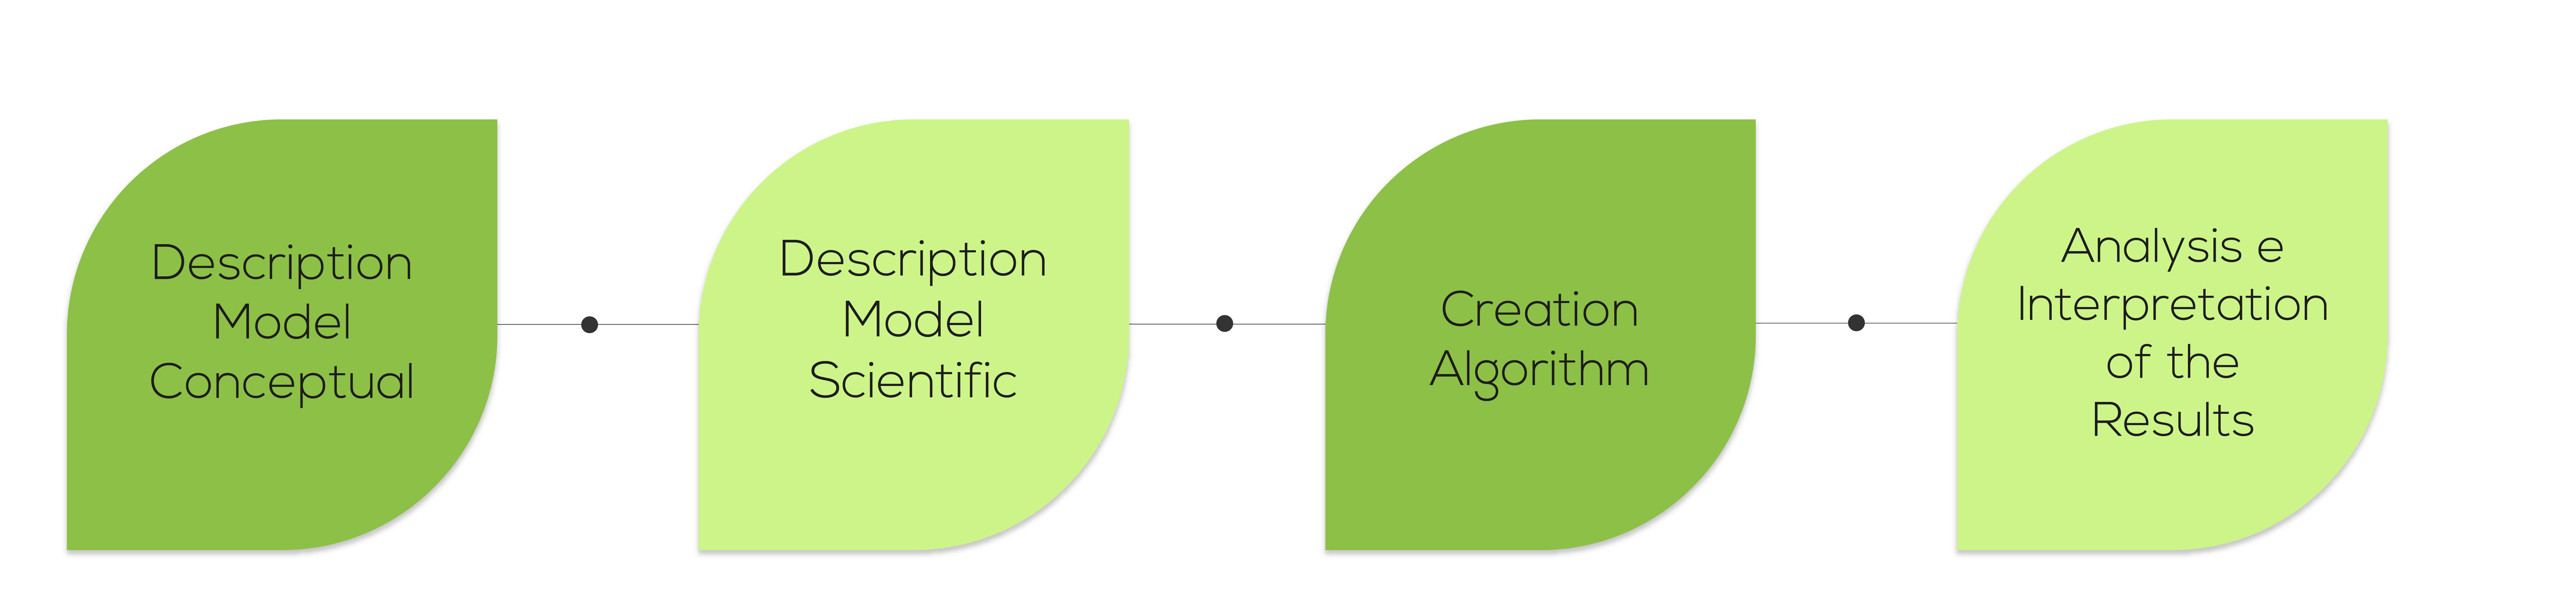
\includegraphics[width=1.1\linewidth]{images/methodologyflow.png}
  \caption{\label{fig:methodologyflow}Timetabling problem methodology}
\end{figure}
\end{slide}


\begin{slide}
\textbf{Methodology:}\\

\begin{figure}[h!]
  \centering
  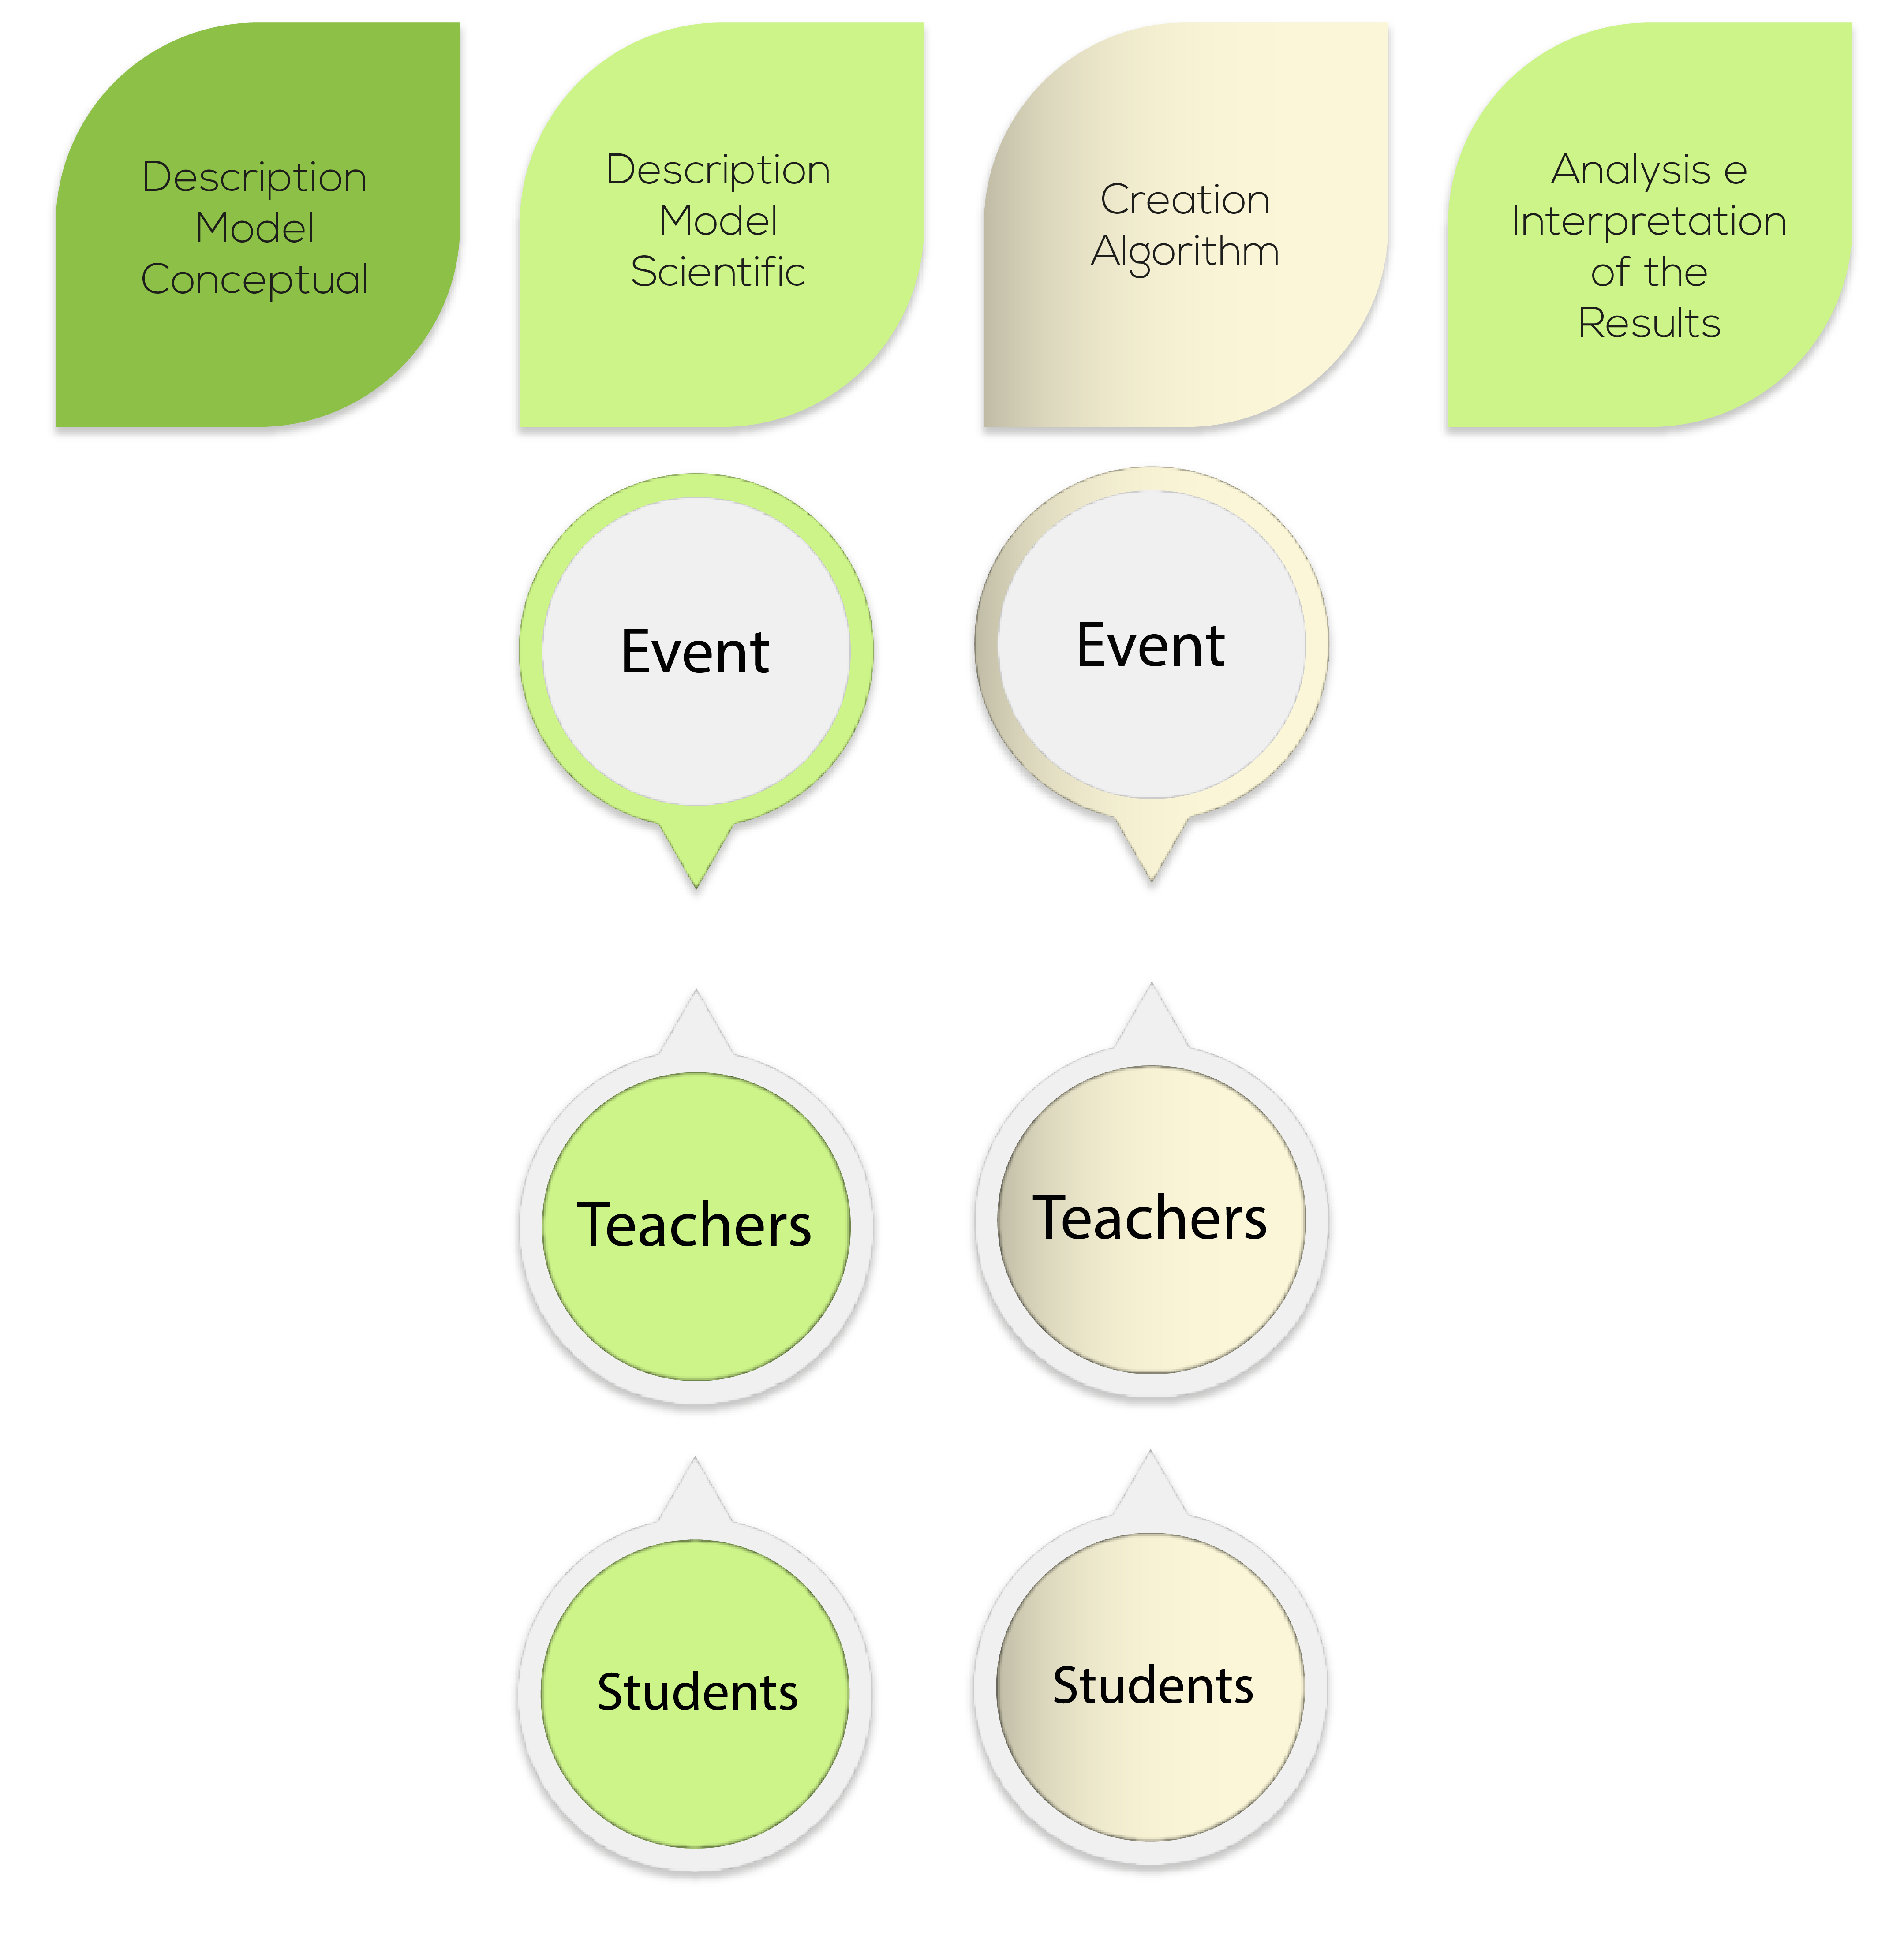
\includegraphics[width=0.7\linewidth]{images/methodologyflow2.png}
  \caption{\label{fig:methodologyflow2}Timetabling problem methodology}
\end{figure}
\end{slide}

\begin{slide}
\textbf{Related work:}\\

\begin{table}[h!]
  \centering
  \resizebox{\textwidth}{!}{%
  \begin{tabular}{| l | l | l |}
    \hline
    \multicolumn{2}{|c|}{\color{black} \textbf{Techniques}} & \color{black} \textbf{Article name} \\ \hline
    \multicolumn{3}{p{10cm}}{} \\
    \hline

    \multicolumn{2}{|l|}{Graph Coloring (GC)} & \color{black} An Introduction to
TimeTabling \cite{DeWerra1985} \\

    \multicolumn{1}{|l}{Integer/Linear
    Programming (IP/LP)} &  \multicolumn{1}{l|}{} & \color{black} \multirow{3}{11cm}{ New integer linear programming approaches for course timetabling \cite{Boland2008} , Integer programming methods for large-scale practical classroom assignment problems \cite{Phillips2015}}\\
    \multicolumn{1}{|l}{}& \multicolumn{1}{l|}{} & \\
    \multicolumn{1}{|l}{}& \multicolumn{1}{l|}{} & \\

    \multicolumn{1}{|l}{Constraint Satisfaction
Programming (CSP)} & \multicolumn{1}{l|}{} & \color{black} Timetable planning using the constraint-based reasoning \cite{Deris2000}\\

    \multicolumn{1}{|l}{Multi-population} & \multicolumn{1}{l|}{\color{black}Genetic Algorithm (GA)} & \color{black} \multirow{2}{11cm}{ A Utilization-based Genetic Algorithm for Solving the University Timetabling Problem (UGA) \cite{Abdelhalim2016} }\\
    \multicolumn{1}{|l}{}& \multicolumn{1}{l|}{} & \\

    \multicolumn{1}{|l}{} & \multicolumn{1}{l|}{\color{black}Ant Colony Optimization (ACO)} & \color{black} \multirow{3}{11cm}{A MAX - MIN Ant System for the University Course Timetabling Problem \cite{Socha2002}, A MAX-MIN Ant System for the University Course Timetabling Problem \cite{Brabazon2015}}\\
    \multicolumn{1}{|l}{}& \multicolumn{1}{l|}{} & \\
    \multicolumn{1}{|l}{}& \multicolumn{1}{l|}{} & \\

    \multicolumn{1}{|l}{} & \multicolumn{1}{l|}{\color{black}Artificial Bee Colony (ABC)} & \color{black} \multirow{2}{11cm}{ University course timetabling using hybridized artificial bee colony with hill climbing optimizer \cite{Bolaji2014}}\\
    \multicolumn{1}{|l}{}& \multicolumn{1}{l|}{} & \\

    \multicolumn{1}{|l}{} & \multicolumn{1}{l|}{\color{black}Memetic Algorithm (MA)} & \color{black} \multirow{2}{11cm}{ Using improved memetic algorithm and local search to solve university Course Timetabling problem (UCTP) \cite{Joudaki2011}}\\
    \multicolumn{1}{|l}{}& \multicolumn{1}{l|}{} & \\

    \multicolumn{1}{|l}{} & \multicolumn{1}{l|}{\color{black}Harmony Search Algorithm (HSA)} & \color{black} \multirow{2}{11cm}{ University course timetabling using a hybrid harmony search metaheuristic algorithm \cite{Al-Betar2012} }\\
    \multicolumn{1}{|l}{}& \multicolumn{1}{l|}{} & \\

    \multicolumn{1}{|l}{Single-population} & \multicolumn{1}{l|}{\color{black}Local Search (LS)} & \color{black} \multirow{4}{11cm}{ A fuzzy genetic algorithm with local search for university course timetabling \cite{Kohshori2011}, Genetic algorithms with guided and local search strategies for university course timetabling \cite{Yang2011}}\\
    \multicolumn{1}{|l}{}& \multicolumn{1}{l|}{} & \\
    \multicolumn{1}{|l}{}& \multicolumn{1}{l|}{} & \\
    \multicolumn{1}{|l}{}& \multicolumn{1}{l|}{} & \\

    \multicolumn{1}{|l}{} & \multicolumn{1}{l|}{\color{black}Variable Neighborhood Search (VNS)} & \color{black} \multirow{2}{11cm}{ An Investigation Of Variable Neighbourhood Search For University Course Timetabling \cite{Abdullah2005}}\\
    \multicolumn{1}{|l}{}& \multicolumn{1}{l|}{} & \\

    \multicolumn{1}{|l}{} & \multicolumn{1}{l|}{\color{black}Simulated Annealing (SA)} & \color{black} \multirow{4}{11cm}{ Solving the Course Scheduling Problem Using Simulated Annealing \cite{Aycan2009}, A hybrid simulated annealing with Kempe Chain neighborhood for the university timetabling problem \cite{Tuga2007}}\\
    \multicolumn{1}{|l}{}& \multicolumn{1}{l|}{} & \\
    \multicolumn{1}{|l}{}& \multicolumn{1}{l|}{} & \\
    \multicolumn{1}{|l}{}& \multicolumn{1}{l|}{} & \\

    \multicolumn{1}{|l}{} & \multicolumn{1}{l|}{\color{black}Tabu Search (TS)} & \color{black} \multirow{4}{11cm}{ The effect of neighborhood structures on tabu search algorithm in solving course timetabling problem \cite{Aladag2009}, Design and implementation of a course scheduling system using Tabu Search \cite{Alvarez-Valdes2002}}\\
    \multicolumn{1}{|l}{}& \multicolumn{1}{l|}{} & \\
    \multicolumn{1}{|l}{}& \multicolumn{1}{l|}{} & \\
    \multicolumn{1}{|l}{}& \multicolumn{1}{l|}{} & \\

    \multicolumn{1}{|l}{Novel Intelligent} & \multicolumn{1}{l|}{\color{black}Hybrid Algorithms (Hybrid Metaheuristic)} & \color{black} \multirow{2}{11cm}{ A new hybrid algorithm for university course timetabling problem using events based on groupings of students \cite{Badoni2014} } \\
    \multicolumn{1}{|l}{}& \multicolumn{1}{l|}{} & \\


    \multicolumn{1}{|l}{} & \multicolumn{1}{l|}{\color{black}Fuzzy method} & \color{black} \multirow{2}{11cm}{Fuzzy genetic heuristic for university course timetable problem \cite{Chaudhuri2010}, A fuzzy solution based on Memetic algorithms for timetabling \cite{Golabpour2008}}\\
    \multicolumn{1}{|l}{}& \multicolumn{1}{l|}{} & \\
    \multicolumn{1}{|l}{}& \multicolumn{1}{l|}{} & \\

    \multicolumn{1}{|l}{} & \multicolumn{1}{l|}{\color{black}Clustering Algorithms} & \color{black} \multirow{2}{11cm}{Applying a novel clustering technique based on FP- tree to University timetabling problem: A case study \cite{Shatnawi2010}}\\
    \multicolumn{1}{|l}{}& \multicolumn{1}{l|}{} & \\


    \multicolumn{1}{|l}{Multi-Agent Systems} & \multicolumn{1}{l|}{ \color{black}Review papers Multi-Agent Systems} & \color{black} \multirow{3}{11cm}{A multi-agent system for course timetabling \cite{Yanga2011}, Implementation of class timetabling using multi agents \cite{Nandhini2009}}\\
    \multicolumn{1}{|l}{}& \multicolumn{1}{l|}{} & \\
    \multicolumn{1}{|l}{}& \multicolumn{1}{l|}{} & \\
  \hline 
  \end{tabular}%
  }
  \label{Table:relatedwork}
  \caption{Brief literature about University Timetabling Problem}
\end{table}
\end{slide}
\begin{slide}
\textbf{Problem formulation:}\\

\begin{table}[h!]
  \centering
  \resizebox{\textwidth}{!}{%
  \begin{tabular}{| l | l |}
    \hline
    \color{black} \textbf{Symbols} & \color{black} \textbf{Definition} \\ \hline
    \multicolumn{2}{p{10cm}}{\color{gray}Sets} \\
    \hline
    $s \in S$ & \color{black}Set of slot composed of days $D$ and periods $P$\\
    $r \in R$ & \color{black}Set of rooms \\
    $e \in E$ & \color{black}Set of event composed of courses $C$ and groups $G$ \\ 
    \hline
    \multicolumn{2}{p{10cm}}{\color{gray}Parameters} \\
    \hline
    $w_{r}$ & \color{black}Unit cost of using the room $r$\\
    $f_e$ & \color{black}frequency with which an event $e$ is given in the week\\
    $dem_e$ & \color{black}Intensity in hours with which an $e$ event is imparted in a day\\
    $cap_s$ & \color{black}Capacity in hours the slot $s$ has\\
    $com_{er}$ & $\left\{
    \begin{array}{l l}
     {\color{black}1} \hspace{1cm} \textrm{{\color{black}if the event} $e$ {\color{black}can be assigned to the room} $r$} \\
     \color{black}0 \hspace{1cm} \textrm{Otherwise}.
    \end{array}
    \right.
    $\\
    $\phi_s$ & \color{black}Subset of incompatible slots with slot $s$ \\
    \hline
    \multicolumn{2}{p{10cm}}{\color{gray}Decision variables} \\
    \hline 
    $x_{esr}$ & $\left\{
    \begin{array}{l l}
     {\color{black}1} \hspace{1cm} \textrm{{\color{black}if the event} $e$ {\color{black}is programmed to a time slot} $s$ {\color{black} that is assigned to the room } $r$} \\
     \color{black}0 \hspace{1cm} \textrm{Otherwise}.
    \end{array}
    \right.
    $\\
    \hline
  \end{tabular}%
  }
  \label{Table:modelevent}
  \caption{Notation used for modeling events at EAFIT University}
\end{table}

\end{slide}

\begin{slide}
\textbf{Model:}\\

\numberwithin{equation}{subsection}
\renewcommand\theequation{\arabic{equation}}


{\LARGE
The objective (\ref{eq:fo}) is to minimize the use of artificial salons. The IP restrictions are described below:

  \begin{align}
    \label{eq:fo} \min \, \sum_{e \in E} \sum_{s \in S} \sum_{r \in R} w_{r} \cdot x_{esr}
  \end{align}
}
\emph{s. t.}

{\LARGE
  \begin{align}
    \label{eq:H1} \sum_{e\,\in\,E}{x_{esr}} \le 1, & \quad \forall \ s\,\in\,S, \ r\,\in \,R \\
    %
    \label{eq:H2} \sum_{r\,\in\,R}{\sum_{s\,\in\,S}{x_{esr}} = f_e}, & \quad \forall \ e\in E \\
    %
    \label{eq:H3} x_{esr}  \le com_{er}, & \quad \forall \ e\in E, \ s\,\in \,S , \ r\,\in \,R \\
    %
    \label{eq:H4} \sum_{e\,\in\,E}{\, \sum_{s'\,\in\,\phi(s)}{x_{es'r}}}  \le 1, & \quad \forall \ r\,\in \,R ,  \ s\,\in \,S \\
    %
    \label{eq:H5} M \cdot ( x_{esr} -1 ) \le -\frac{dem_e}{cap_s} + 1, & \quad \forall \ e\in E, \ s\,\in \,S , \ r\,\in \,R
  \end{align}
}

\end{slide}

\begin{slide}
\textbf{Constraints:}\\

\begin{itemize}
\item \ref{eq:H1} - satisfies the restriction $HC_1$.
\item \ref{eq:H2} - satisfies the restriction $HC_3$.
\item \ref{eq:H3} - satisfies the restriction $HC_2$.
\item \ref{eq:H4} - only one event can be assigned to one of the slots of the subset of incompatible slots $\phi_s$.
\item \ref{eq:H5} - satisfies the restriction $HC_4$.
\end{itemize}

\end{slide}

\begin{slide}
\textbf{Algorithmic solution:}\\

\begin{figure}[h!]
  \centering
  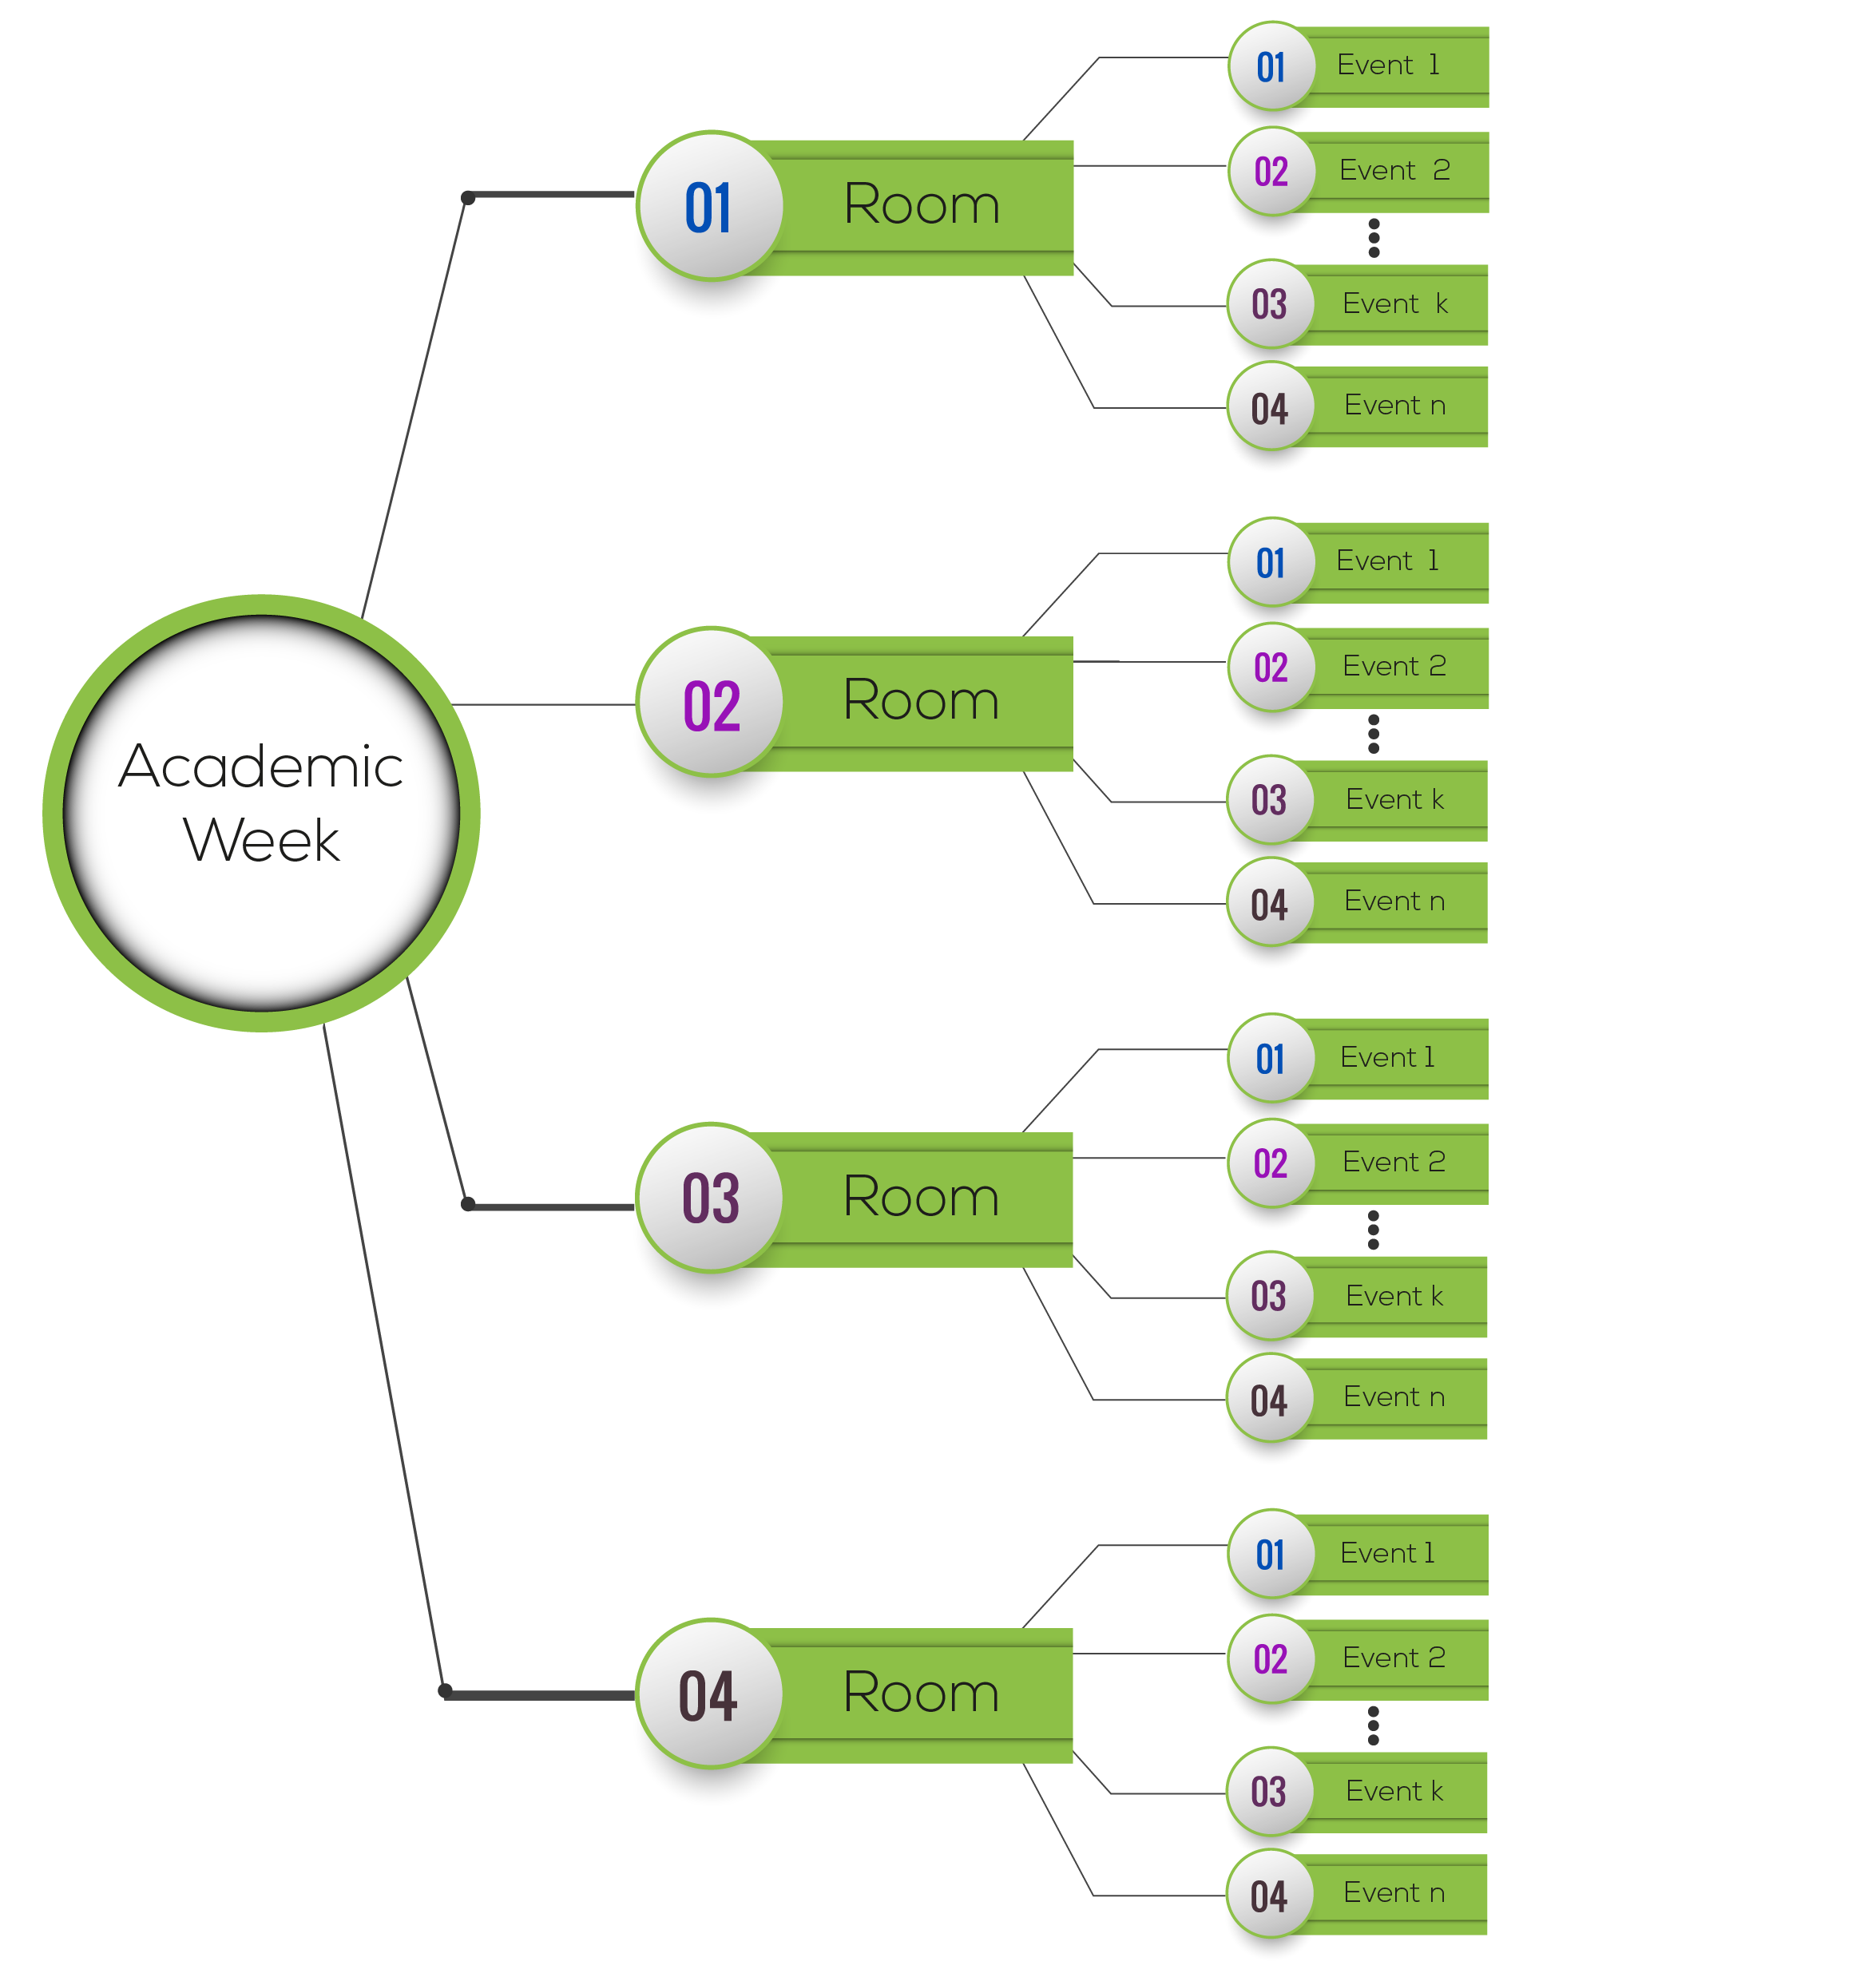
\includegraphics[width=0.65\linewidth]{images/chainresponsability.png}
  \caption{\label{fig:methodologyflow2}Chain Responsability to Timetabling problem}
\end{figure}
\end{slide}

\begin{slide}
\textbf{Algorithmic solution:}\\

{\huge
  \begin{algorithmic}[1]
    \Procedure{GRASP Metaheurístic}{}%\Comment{The g.c.d. of a and b}
    \State $f^* \gets \alpha $
    \State $input \gets $ \textbf{ReadInput()};
    \If{ \textbf{validate($ input $)} }
      \For{$i \leq i_{max}$}
        \State $x\gets $ \textbf{GreedyRandomized()};
        \State $x\gets $ \textbf{LocalSearch($x$)};
        \If{ $f(x) < f^*$ }
          \State $f^*\gets f(x);$
          \State $x^*\gets x;$
        \EndIf    
      \EndFor
    \EndIf
    \State \textbf{WriteOutput($x^*$)};%\Comment{The gcd is b}
    \EndProcedure
  \end{algorithmic}
}
\end{slide}

\begin{slide}
\textbf{Computational experiments:}\\

According to \citep{Bolaji2014, eventMAP} the algorithm will be tested using the following instances:\\

  \begin{table}[h!]
  \centering
  \resizebox{\textwidth}{!}{%
  \begin{tabular}{| l | l | l | l |}
    \hline
    \color{black}Instance & \color{black}small & \color{black}\color{black}medium  & \color{black}large\\ \hline \hline
    \color{black}Events & 100 & 400 & 400 \\
    \color{black}Room & 5 & 5 &  10 \\
    \color{black}Day & 5 & 5 & 5 \\
    \color{black}Slot & 8 & 8 & 8 \\
    \hline
  \end{tabular}%
  }
  \label{Table:instances}
  \caption{Set of test instances at EAFIT University}
\end{table}

\end{slide}

\begin{slide}
\textbf{Computational experiments:}\\
\begin{table}[h!]
  \centering
  \resizebox{\textwidth}{!}{%
  \begin{tabular}{| l | l | l | l | l | l | l | l | l |}
    \hline
    \color{black}\textbf{Room}&\color{black}\textbf{Type Room}&\color{black}\textbf{Capacity}&\color{black}\textbf{Event}&\color{black}\textbf{Group}&\color{black}\textbf{Max Student}&\color{black}\textbf{Day}&\color{black}\textbf{Start Time}&\color{black}\textbf{End Time} \\ \hline \hline

    \color{black}35401&\color{black}Aula Normal&\color{black}50&\color{black}METODOLOGÍA DEL APRENDIZAJE&\color{black}024 & \color{black}26 & \color{black}T  & \color{black}7.0 & \color{black}9.0 \\
    \color{black}35401 & \color{black}Aula Normal & \color{black}50 & \color{black}MODELACIÓN Y SIMULACIÓN I & \color{black}001 & \color{black}30 & \color{black}T  & \color{black}9.0 & \color{black}12.0 \\
    \color{black}35401 & \color{black}Aula Normal & \color{black}50 & \color{black}METODOLOGÍA DEL APRENDIZAJE & \color{black}024 & \color{black}26 & \color{black}W  & \color{black}14.0 & \color{black}15.0 \\
    \color{black}35401 & \color{black}Aula Normal & \color{black}50 & \color{black}MATEMÁTICAS I & \color{black}002 & \color{black}40 & \color{black}TH  & \color{black}18.0 & \color{black}21.0 \\
    \color{black}35401 & \color{black}Aula Normal & \color{black}50 & \color{black}MATEMÁTICAS 1 & \color{black}010 & \color{black}37 & \color{black}F  & \color{black}6.0 & \color{black}9.0 \\
    \color{black}35403 & \color{black}Aula Normal & \color{black}36 & \color{black}MATEMÁTICAS III (ECONOMÍA) & \color{black}003 & \color{black}32 & \color{black}F  & \color{black}6.0 & \color{black}9.0 \\
    \color{black}35501 & \color{black}Aula Normal & \color{black}50 & \color{black}BIOLOGÍA MOLECULAR & \color{black}101 & \color{black}30 & \color{black}F  & \color{black}6.0 & \color{black}9.0 \\
    \color{black}35501 & \color{black}Aula Normal & \color{black}50 & \color{black}MATEMÁTICAS 1 & \color{black}001 & \color{black}37 & \color{black}S  & \color{black}12.0 & \color{black}15.0 \\
    \color{black}38107 & \color{black}Aula Normal & \color{black}25 & \color{black}FUNDAMENTOS DE FISICOQUÍMICA & \color{black}156 & \color{black}20 & \color{black}T  & \color{black}15.0 & \color{black}17.0 \\
    \color{black}38107 & \color{black}Aula Normal & \color{black}25 & \color{black}FUNDAMENTOS DE FISICOQUÍMICA & \color{black}156 & \color{black}20 & \color{black}S  & \color{black}9.0 & \color{black}12.0 \\
    \color{black}38201 & \color{black}Aula Normal & \color{black}50 & \color{black}BIOÉTICA & \color{black}001 & \color{black}30 & \color{black}M  & \color{black}6.0 & \color{black}8.0 \\
    \color{black}38201 & \color{black}Aula Normal & \color{black}50 & \color{black}METODOLOGÍA DEL APRENDIZAJE & \color{black}022 & \color{black}26 & \color{black}W  & \color{black}14.0 & \color{black}15.0 \\
    \color{black}38201 & \color{black}Aula Normal & \color{black}50 & \color{black}ESTADÍSTICA 2 (ECONOMÍA) & \color{black}001 & \color{black}26 & \color{black}W  & \color{black}9.0 & \color{black}12.0 \\
    \color{black}38201 & \color{black}Aula Normal & \color{black}50 & \color{black}BIOÉTICA & \color{black}001 & \color{black}30 & \color{black}F  & \color{black}11.0 & \color{black}12.0 \\


    \hline
  \end{tabular}%
  }
  \label{Table:result}
  \caption{Timetabling Events at EAFIT University}
\end{table}
\end{slide}

\begin{slide}
\textbf{Conclusions:}\\

\begin{itemize}
\item The first stage of the problem was successfully modeled, which corresponds to the assignment of events.
\item An algorithm was proposed for the scheduling of events
at the EAFIT University.
\item An algorithm was proposed for the scheduling of teacher
at the EAFIT University.
\end{itemize}
\end{slide}

% ---------------------------------------------------------------------
% -- References --
% ---------------------------------------------------------------------
%\begin{slide}
%\textbf{\color{darkred} References}

%\end{slide}
% ---------

\begin{frame}\\
  \bibliographystyle{authordate1}
  %\bibliographystyle{alpha}
  \large{\bibliography{bibliography.bib}}
\end{frame}

\begin{slide}
(Bonus Slides)
\end{slide}
% ---------


\begin{slide}
\textbf{Solution construction flow:}\\
{\huge
  \begin{algorithmic}[1]
    \Procedure{GreedyRandomized}{}%\Comment{The g.c.d. of a and b}

    \State $teacher \gets $ \textbf{SetOutData( \textbf{GetInData($event$)})};
    \State $event \gets $ \textbf{SetNext($teacher$)};
    \State $room \gets $ \textbf{SetOutData( \textbf{GetInData($event$)} )};
    \State $room \gets $ \textbf{SetNext($event$)};

    \State $slot \gets $ \textbf{SetSlotFree( \textbf{GetInData($slot$)} )};
    \State $slot \gets $ \textbf{SetOutData( \textbf{GetInData($room$)} )};
    \State $slot \gets $ \textbf{SetNext($room$)};
    \State \textbf{processor($slot$)};

    \EndProcedure
  \end{algorithmic}
}
\end{slide}


\begin{slide}
\textbf{Processor:}\\
{\huge
  \begin{algorithmic}[1]
    \Procedure{Processor}{}%\Comment{The g.c.d. of a and b}

    \State \textbf{MakeObject($inData$)};
    \If{ \textbf{ Next()} $\not= null$}
      \State \textbf{Next().processor()}
    \EndIf
    \EndProcedure
  \end{algorithmic}
}
\end{slide}

\end{document}
